\section{Uniform Dynamics - 均匀动力演化}
From the time-dependent Schr\"odinger's Equation, it induces unitary evolution in a quantum system (which in converse, derives the Schr\"odinger's Equation), which is described by a unitary propagator in the form:
$$\opuni(t_2, t_1) \ket{\psi(t_1)} = \ket{\psi(t_2)}$$
\begin{definition}
    \uimpt{Uniform dynamics} is a term that describes unitary evolution. \\
    A unitary evolution is \uimpt{uniform} if
    $$\forall t_1, t_2, \opuni(t_2, t_1) = \opuni(t_2 - t_1, 0)$$
    i.e. the propagator only depends on the time difference $\Delta t= t_2 - t_1$
\end{definition}
Notation-wise, if an evolution is uniform, we write:
$$\opuni(t_2, t_1) = \opuni(t_2 - t_1)$$
\begin{theorem}
    A unitary evolution is uniform if and only if the associated Hamiltonian is time-independent ($\hamiltonian(t) \equiv \hamiltonian$).
\end{theorem}
Intuitively, if we start at the time-dependent Schr\"odinger's Equation, we should have:
\begin{align*}
    \imag \hbar \pdv{t}\ket{\psi(t)} &= \hamiltonian(t) \ket{\psi(t)} \\
    \pdv{t} \ket{\psi(t)} &= \frac{1}{\imag \hbar} \hamiltonian(t) \ket{\psi(t)} \\
    \Delta \ket{\psi(t)} & \approx \Delta t \cdot \frac{1}{\imag \hbar} \hamiltonian(t) \ket{\psi(t)}
\end{align*}
Then, if we wish that the evolution of the state is only dependent on the time difference ($\Delta t$), the Hamiltonian should be time-independent.
\subsection{Proof of Uniform Dynamics associates with a Time-independent Hamiltonian}
We first observe the following for uniform dynamics:
$$\opuni(\Delta t)\opuni(\Delta s)\ket{\psi(t)} = \opuni(\Delta t)\ket{\psi(t + \Delta s)} = \ket{\psi(t + \Delta s + \Delta t)} = \opuni(\Delta s + \Delta t)\ket{\psi(t)}$$
This gives the lemma
\begin{lemma}
    Let $\opuni(\cdot)$ be uniform, then
    $$\forall \ket{\psi(t)}\in\hilbert, \opuni(\Delta t)\opuni(\Delta s) = \opuni(\Delta t + \Delta s)$$
\end{lemma}
This gives us
$$\opuni(\Delta t)\opuni(\Delta t)\dots\opuni(\Delta t) = \opuni(\Delta t)^m = \opuni(m\cdot \Delta t)$$
Since $\opuni$ has some orthonormal eigenbasis $\{\ket{k}\}_k$, we know $\opuni^m$ has the \impt{same} orthonormal eigenbasis, and it remains same for all $m \in \N, \Delta t \in \R$. This thus shows the eigenbasis of $\opuni$ is independent of $\Delta t$, remains constant over time. Hence, we can express $\opuni(\Delta t)$ as the following forms:
\begin{align*}
    \opuni(\Delta t) &= \Sumi{k} \lambda_k(\Delta t) \dyad{k} \\
    &= \Sumi{k} e^{\imag \alpha_k(\Delta t)} \dyad{k}
\end{align*}
Since, we have $\opuni(\Delta t)^m = \opuni(m\cdot \Delta t)$, we have:
\begin{align*}
    \Sumi{k}(e^{\imag \alpha_k(\Delta t)})^m \dyad{k} &= \Sumi{k} e^{\imag \alpha_k(m\Delta t)} \dyad{k} \\
    m \cdot \alpha_k(\Delta t) &= \alpha_k(m \Delta t)
\end{align*}
This immediately shows that $\alpha_k$ is linear, and we can write it in the form of:
$$\alpha_k(\Delta t) = -\omega_k \cdot \Delta t$$
At this intermediate step, suppose that the initial state is an eigenstate of $\opuni(\Delta t)$, that is $\ket{\psi(0)} = \ket{k}$, then we must have:
$$\ket{\psi(t)} = \opuni(t)\ket{\psi(0)} = \Sumi{l}e^{\imag \alpha_l(t)}\dyad{l} \ket{k} = e^{\imag \alpha_k(t)}\ket{k} = e^{-\imag \omega_k t}\ket{k}$$
Notice that with respect to the initial state, it has only evolved with a global phase, that is $\abs{e^{-\imag \omega_k t}} = 1$, the direction of the state remains unchanged.
\begin{definition}
    Quantum states that only evolve with a global phase are \uimpt{stationary states}.
\end{definition}
However, even though stationary states only evolve with a global phase, for each state, there will be a different $\omega_k$ that essentially determines the angular velocity at which it ``rotates''. \par
We then insert this intermediate conclusion into the Schr\"odinger's Equation with a general $\hamiltonian(t)$:
\begin{align*}
    \hamiltonian(t)\ket{\psi(t)} &= \imag \hbar \pdv{t}\ket{\psi(t)} \\
    \hamiltonian(t)(e^{-\imag \omega_k t}\ket{k}) &= \imag \hbar \pdv{t}(e^{-\imag \omega_k t}\ket{k}) \\
    e^{-\imag \omega_k t}\hamiltonian(t)\ket{k} &= \imag \hbar (-\imag \omega_k)(e^{-\imag \omega_k t}\ket{k}) \\
    \hamiltonian(t)\ket{k} &= \hbar \omega_k \ket{k}
\end{align*}
We can thus conclude that:
\begin{quote}
    1. The eigenstates of $\opuni(\Delta t)$ are also eigenstates of the Hamiltonian. \\
    2. The eigenvalues of $\hamiltonian(t)$ are $\hbar \omega_k =: E_k$, which are constant.
\end{quote}
With these two conclusions, we finally can claim that $\hamiltonian(t)$ is a constant operator independent of time:
$$\hamiltonian(t) \equiv \hamiltonian \equiv \Sumi{k}E_k\dyad{k}$$

\subsection{Proof of Time-independent Hamiltonian reflects Uniform Dynamics}
If the Hamiltonian is time-independent, we can write the Hamiltonian in the form:
$$\hamiltonian = \Sumi{k}E_k \dyad{k}$$
where $\{\ket{k}\}_k$ is the orthonormal eigenbasis of the Hamiltonian. \par
Consider an arbitrary state, expressed in this basis, we have:
$$\ket{\psi(t)} = \Sumi{k}c_k(t) \ket{k}$$
Then, the Schr\"odinger's Equation implies:
\begin{align*}
    \hamiltonian\ket{\psi(t)} &= \imag \hbar \pdv{t}\ket{\psi(t)} \\
    \hamiltonian (\Sumi{k}c_k(t) \ket{k}) &= \imag \hbar \pdv{t}(\Sumi{k}c_k(t) \ket{k}) \\
    \Sumi{k}c_k(t) \hamiltonian \ket{k} &= \imag \hbar \Sumi{k}c_k^{'}(t) \ket{k} \\
    \Sumi{k}c_k(t) E_k \ket{k} &= \Sumi{k} \imag \hbar c_k^{'}(t) \ket{k}
\end{align*}
Component-wise, with each summand, we have:
$$c_k(t) E_k = \imag \hbar c_k^{'}(t)$$
which is a differential equation with the solution:
$$c_k(t) = C_k^{(0)}\exp(\frac{E_k t}{\imag \hbar}) = C_k^{(0)}\exp(-\imag \frac{E_k t}{\hbar})$$
where $C_k^{(0)}$ is the initial condition. \par
Here, we know the time evolution of an arbitrary state under the time-independent Hamiltonian:
$$\ket{\psi(t)} = \Sumi{k} C_k^{(0)}\exp(-\imag \frac{E_k t}{\hbar}) \ket{k}$$
We choose the unitary propagator of this time evolution to be:
$$\opuni(\Delta t) = \Sumi{k} e^{-\imag \omega_k t}\dyad{k}$$
where $\omega_k = \frac{E_k}{\hbar}$, this propagator is uniform by design. We then show that this indeed is the desired propagator.
\begin{align*}
    \opuni(\Delta t)\ket{\psi(t)} &= (\Sumi{l} \exp(-\imag \omega_l \Delta t) \dyad{l})(\Sumi{k} C_k^{(0)}\exp(-\imag \omega_k t) \ket{k}) \\
    &= \Sumi{k} C_k^{(0)} \exp(-\imag \omega_k (t + \Delta t)) \ket{k} \\
    &= \ket{\psi(t+\Delta t)}
\end{align*}
In a continuous space, we also have:
\begin{align*}
    \opuni(\Delta t)\ket{\psi(t)} &= \intR \exp(-\imag \omega_y \Delta t) \dyad{y} \dd y \intR C_k^{(0)} \exp(-\imag \omega_x t) \ket{x} \dd x \\
    &= \intR\intR C_k^{(0)} \exp(-\imag \omega_x t) \exp(-\imag \omega_y \Delta t) \ket{y}\braket{y}{x} \dd x \dd y \\
    &= \intR C_k^{(0)} \exp(-\imag \omega_x t) \exp(-\imag \omega_x \Delta t) \ket{x} \dd x \\
    &= \ket{\psi(t+\Delta t)}
\end{align*}

\subsection{Intermediate Summary}
To summarize, for uniform dynamics, the Schr\"odinger's Equation is reduced to the eigenvalue problem:
$$\hamiltonian\ket{k} = E_k \ket{k}$$
which is also the \impt{time-independent Schr\"odinger's Equation}. After solving the eigenvalue problem, we will be able to find $\{E_k\}_k$ and $\{\ket{k}\}_k$. \par
We would also know the unitary propagator to be:
$$\opuni(\Delta t) = \Sumi{k} e^{-\imag \omega_k t}\dyad{k}$$
where $\omega_k = \frac{E_k}{\hbar}$, and the eigenstates of the propagator are \impt{stationary states}:
$$\opuni(t)\ket{k} = e^{-\imag \omega_k t}\ket{k}$$
And, for an arbitrary state, the time evolution is:
$$\ket{\psi(t)} = \Sumi{k} C_k^{(0)}\exp(-\imag \omega_k t) \ket{k}$$

\subsection{Rotation on the Bloch Sphere - 量子态在布洛赫球面的旋转}
Consider an example of a Hamiltonian being the following:
$$\hamiltonian = EX = \begin{pmatrix}
    0 & E \\
    E & 0
\end{pmatrix}$$
where $E \in \R$, and the eigenbasis of the Hamiltonian is the same as that of Pauli-X: $\{\ketplus, \ketminus\}$. We know that
$$X = \dyad{+} - \dyad{-}$$
then, we have
$$\hamiltonian = (+E)\ketbra{+}{+} + (-E)\ketbra{-}{-}$$
Recall that for uniform dynamics, if $\displaystyle \hamiltonian = \Sumi{k}E_k \dyad{k}$, then the unitary propagator is represented by $\displaystyle \opuni(t) = \Sumi{k}e^{-\imag \omega_k t} \dyad{k}$, where $\omega_k = \frac{E_k}{\hbar}$. Thus, in this case, the unitary propagator is:
$$\opuni(t) = \exp(-\imag \frac{E}{\hbar} t)\dyad{+} + \exp(\imag \frac{E}{\hbar} t)\dyad{-}$$
Suppose the initial state $\ket{\psi(0)} = \ket{0} = \frac{\ketplus + \ketminus}{\sqrt{2}}$, we have:
\begin{align*}
    \ket{\psi(t)} &= \frac{1}{\sqrt{2}}(\exp(-\imag \frac{E}{\hbar} t)\ketplus + \exp(\imag \frac{E}{\hbar} t)\ketminus) \\
    &= \cos(\frac{Et}{\hbar})\ket{0} - \imag \cdot \sin(\frac{Et}{\hbar})\ket{1}
\end{align*}
The evolution reflects the rotation in the Bloch sphere around the axis through the eigenbasis of $\hamiltonian$, which in this case $\{\ketplus, \ketminus\}$
\begin{center}
    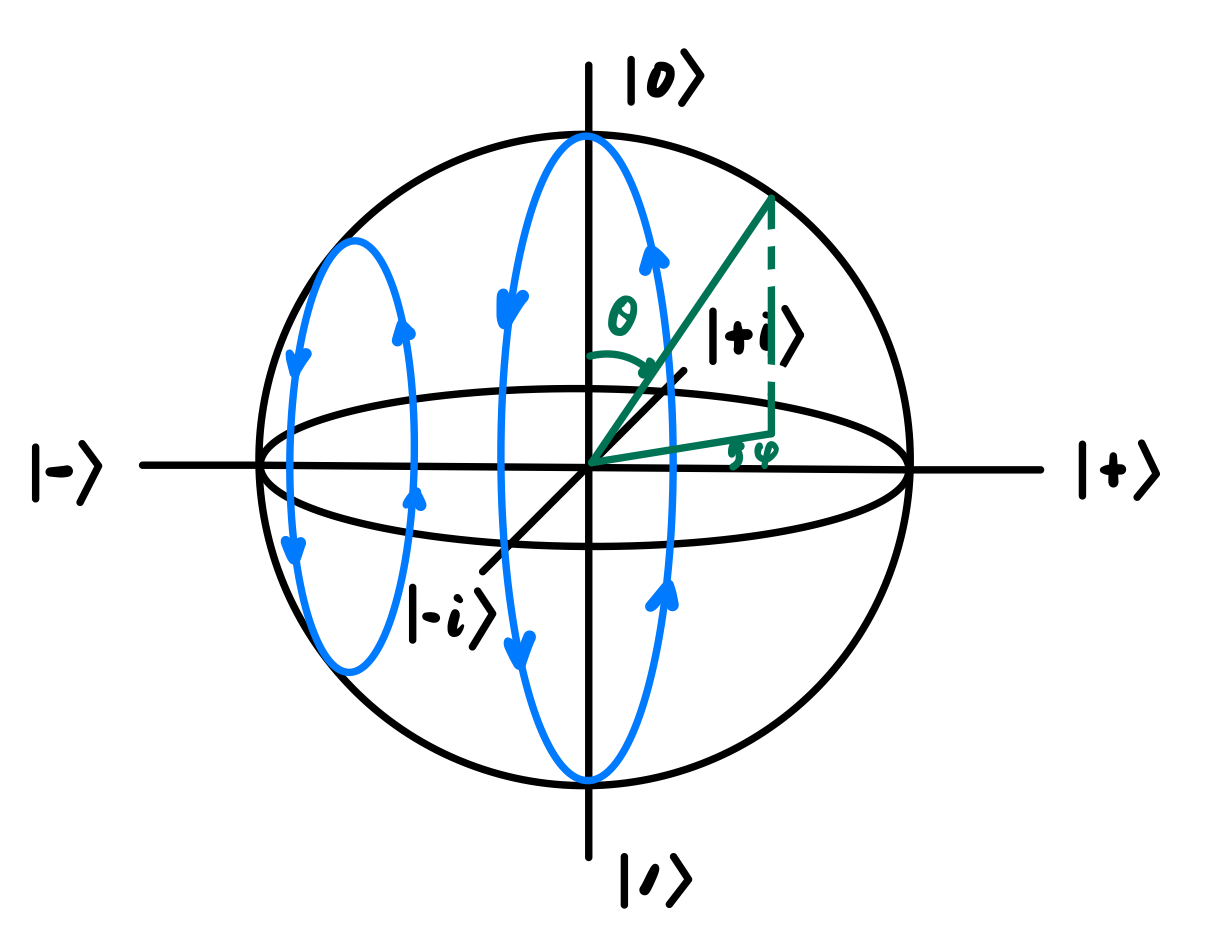
\includegraphics[scale = 0.3]{bloch-sphere-rotation.png}
\end{center}
We may also substitute Pauli-X with other Pauli operators so that the rotation would be in the respective axis.

\subsection{Evolution of Observables and Symmetries - 可观测量的演化和对称性}
From the third postulate, we know for a time-independent observable $A$, which is a Hermitian operator, the expected value of $A$ is:
$$\expval{A}_\psi = \expval{A}{\psi}$$
From this, we wish to understand how does $\expval{A}$ evolve with respect to $\psi$ evolving in time.
\begin{definition}
    Consider an observable $A$ with respect to a state $\ketpsi$, the evolution of this observable in time is
    $$\expval{A}_t := \expval{A}_{\psi(t)} = \expval{A}{\psi(t)}$$
\end{definition}
This further means $\expval{A}_t = \expval{\conjt{\opuni(t)}A\opuni(t)}{\psi(0)}$. \par
Knowing how $\ket{\psi(t)}$ evolves from the fourth postulate, we can look into the time-derivative of the expected value of an observable $A$ over time with respect to a state $\ketpsi$:
\begin{align*}
    \pdv{t} \expval{A}_t &= \pdv{t} \expval{A}{\psi(t)} \\
    &= \bra{\psi(t)}A(\pdv{t}\ket{\psi(t)}) + (\pdv{t}\bra{\psi(t)})A\ket{\psi(t)} \\
    &= \bra{\psi(t)}A(-\frac{\imag}{\hbar} \hamiltonian \ket{\psi(t)}) + (\frac{\imag}{\hbar} \bra{\psi(t)} \conjt{\hamiltonian})A\ket{\psi(t)} \\
    &= \frac{\imag}{\hbar}(\expval{-A\hamiltonian}{\psi(t)} + \expval{\hamiltonian A}{\psi(t)}) \\
    &= \frac{\imag}{\hbar} \expval{\hamiltonian A-A\hamiltonian}{\psi(t)} \\
    &= \frac{\imag}{\hbar} \expval{[\hamiltonian, A]}_t
\end{align*}
\begin{definition}
    An observable $A$ is called a \uimpt{conserved quantity} if
    $$\pdv{t} \expval{A}_t = 0$$
\end{definition}
Equivalently, this means, for time-independent observables $A$, $A$ is \impt{conserved} $\iff$ for all time $t$, $A$ \hyperref[subsec:commutator]{\textcolor{cyan}{commutes with}} $\hamiltonian$, that is, $[\hamiltonian, A] = 0$. Here, a time-independent observable means the projective measurement is independent of time, or, the state is always measured in the same way regardless of time evolution. \par
A trivial example is that $[\hamiltonian, \hamiltonian] = 0$, where as we previously reached that $\hamiltonian$ can be interpreted as an observable such that when measured reflects the total energy of the system, meaning \impt{total energy of a system is conserved}.
\begin{definition}
    A unitary operator $V$ is called a \uimpt{symmetry} if it commutes with the unitary propagator for all times, that is,
    $$[V, \opuni(t)] = 0$$
\end{definition}
Conserved quantities and symmetries imply each other.

\newpage